\documentclass{beamer}
\usetheme{tokitex}

\usepackage{tikz}
\usepackage{graphics}
\usepackage{multirow}
\usepackage{tabto}
\usepackage{xspace}
\usepackage{amsmath}
\usepackage{hyperref}
\usepackage{wrapfig}
\usepackage{mathtools}

\usepackage{tikz}
\usepackage{clrscode3e}
\usepackage{gensymb}

\usepackage[english,bahasa]{babel}
\newtranslation[to=bahasa]{Section}{Bagian}
\newtranslation[to=bahasa]{Subsection}{Subbagian}

\usepackage{listings, lstautogobble}
\usepackage{color}

\definecolor{dkgreen}{rgb}{0,0.6,0}
\definecolor{gray}{rgb}{0.5,0.5,0.5}
\definecolor{mauve}{rgb}{0.58,0,0.82}

\lstset{frame=tb,
  language=c++,
  aboveskip=0mm,
  belowskip=0mm,
  showstringspaces=false,
  columns=fullflexible,
  keepspaces=true,
  basicstyle={\small\ttfamily},
  numbers=none,
  numberstyle=\tiny\color{gray},
  keywordstyle=\color{blue},
  commentstyle=\color{dkgreen},
  stringstyle=\color{mauve},
  breaklines=true,
  breakatwhitespace=true,
  lineskip={-3pt}
}

\usepackage{caption}
\captionsetup[figure]{labelformat=empty}

\newcommand{\progTerm}[1]{\textbf{#1}}
\newcommand{\foreignTerm}[1]{\textit{#1}}
\newcommand{\newTerm}[1]{\alert{\textbf{#1}}}
\newcommand{\emp}[1]{\alert{#1}}
\newcommand{\statement}[1]{"#1"}

\newcommand{\floor}[1]{\lfloor #1 \rfloor}
\newcommand{\ceil}[1]{\lceil #1 \rceil}
\newcommand{\abs}[1]{\left\lvert#1\right\rvert}
\newcommand{\norm}[1]{\left\lVert#1\right\rVert}

% Getting tired of writing \foreignTerm all the time
\newcommand{\farray}{\foreignTerm{array}\xspace}
\newcommand{\fArray}{\foreignTerm{Array}\xspace}
\newcommand{\foverhead}{\foreignTerm{overhead}\xspace}
\newcommand{\fOverhead}{\foreignTerm{Overhead}\xspace}
\newcommand{\fsubarray}{\foreignTerm{subarray}\xspace}
\newcommand{\fSubarray}{\foreignTerm{Subarray}\xspace}
\newcommand{\fbasecase}{\foreignTerm{base case}\xspace}
\newcommand{\fBasecase}{\foreignTerm{Base case}\xspace}
\newcommand{\ftopdown}{\foreignTerm{top-down}\xspace}
\newcommand{\fTopdown}{\foreignTerm{Top-down}\xspace}
\newcommand{\fbottomup}{\foreignTerm{bottom-up}\xspace}
\newcommand{\fBottomup}{\foreignTerm{Bottom-up}\xspace}
\newcommand{\fpruning}{\foreignTerm{pruning}\xspace}
\newcommand{\fPruning}{\foreignTerm{Pruning}\xspace}

\newcommand{\fgraph}{\foreignTerm{graph}\xspace}
\newcommand{\fGraph}{\foreignTerm{Graph}\xspace}
\newcommand{\froot}{\foreignTerm{root}\xspace}
\newcommand{\fRoot}{\foreignTerm{Root}\xspace}
\newcommand{\fnode}{\foreignTerm{node}\xspace}
\newcommand{\fNode}{\foreignTerm{Node}\xspace}
\newcommand{\fedge}{\foreignTerm{edge}\xspace}
\newcommand{\fEdge}{\foreignTerm{Edge}\xspace}
\newcommand{\fcycle}{\foreignTerm{cycle}\xspace}
\newcommand{\fCycle}{\foreignTerm{Cycle}\xspace}
\newcommand{\fdegree}{\foreignTerm{degree}\xspace}
\newcommand{\fDegree}{\foreignTerm{Degree}\xspace}
\newcommand{\fadjacencylist}{\foreignTerm{adjacency list}\xspace}
\newcommand{\fAdjacencylist}{\foreignTerm{Adjacency list}\xspace}
\newcommand{\fadjacencymatrix}{\foreignTerm{adjacency matrix}\xspace}
\newcommand{\fAdjacencymatrix}{\foreignTerm{Adjacency matrix}\xspace}
\newcommand{\fedgelist}{\foreignTerm{edge list}\xspace}
\newcommand{\fEdgelist}{\foreignTerm{Edge list}\xspace}
\newcommand{\flist}{\foreignTerm{list}\xspace}
\newcommand{\fList}{\foreignTerm{List}\xspace}
\newcommand{\fgraphtraversal}{\foreignTerm{graph traversal}\xspace}
\newcommand{\fGraphtraversal}{\foreignTerm{Graph traversal}\xspace}
\newcommand{\ftree}{\foreignTerm{tree}\xspace}
\newcommand{\fTree}{\foreignTerm{Tree}\xspace}
\newcommand{\fsubtree}{\foreignTerm{subtree}\xspace}
\newcommand{\fSubtree}{\foreignTerm{Subtree}\xspace}
\newcommand{\fparent}{\foreignTerm{parent}\xspace}
\newcommand{\fParent}{\foreignTerm{Parent}\xspace}
\newcommand{\fsibling}{\foreignTerm{sibling}\xspace}
\newcommand{\fSibling}{\foreignTerm{Sibling}\xspace}
\newcommand{\fpath}{\foreignTerm{path}\xspace}
\newcommand{\fPath}{\foreignTerm{Path}\xspace}
\newcommand{\fconnectedcomponent}{\foreignTerm{connected component}\xspace}
\newcommand{\fConnectedcomponent}{\foreignTerm{Connected component}\xspace}
\newcommand{\fbridge}{\foreignTerm{bridge}\xspace}
\newcommand{\fBridge}{\foreignTerm{Bridge}\xspace}
\newcommand{\farticulationpoint}{\foreignTerm{articulation point}\xspace}
\newcommand{\fArticulationpoint}{\foreignTerm{Articulation point}\xspace}
\newcommand{\ftreeedge}{\foreignTerm{tree edge}\xspace}
\newcommand{\fTreeedge}{\foreignTerm{Tree edge}\xspace}
\newcommand{\fbackedge}{\foreignTerm{back edge}\xspace}
\newcommand{\fBackedge}{\foreignTerm{Back edge}\xspace}
\newcommand{\fforwardedge}{\foreignTerm{forward edge}\xspace}
\newcommand{\fForwardedge}{\foreignTerm{Forward edge}\xspace}
\newcommand{\fcrossedge}{\foreignTerm{cross edge}\xspace}
\newcommand{\fCrossedge}{\foreignTerm{Cross edge}\xspace}
\newcommand{\fdiscoverytime}{\foreignTerm{discovery time}\xspace}
\newcommand{\fDiscoverytime}{\foreignTerm{Discovery time}\xspace}
\newcommand{\flowlink}{\foreignTerm{low link}\xspace}
\newcommand{\fLowlink}{\foreignTerm{Low link}\xspace}
\newcommand{\fstack}{\foreignTerm{stack}\xspace}
\newcommand{\fStack}{\foreignTerm{Stack}\xspace}
\newcommand{\for}{\foreignTerm{or}\xspace}
\newcommand{\fOr}{\foreignTerm{Or}\xspace}
\newcommand{\fand}{\foreignTerm{and}\xspace}
\newcommand{\fAnd}{\foreignTerm{And}\xspace}
\newcommand{\fcentroid}{\foreignTerm{centroid}\xspace}
\newcommand{\fCentroid}{\foreignTerm{Centroid}\xspace}

\newcommand{\fDivideAndConquer}{\foreignTerm{Divide and conquer}\xspace}
\newcommand{\fdivideAndConquer}{\foreignTerm{divide and conquer}\xspace}
\newcommand{\fMergeSort}{\foreignTerm{Merge sort}\xspace}
\newcommand{\fmergeSort}{\foreignTerm{merge sort}\xspace}
\newcommand{\fQuickSort}{\foreignTerm{Quicksort}\xspace}
\newcommand{\fquickSort}{\foreignTerm{quicksort}\xspace}
\newcommand{\fpivot}{\foreignTerm{pivot}\xspace}
\newcommand{\fPivot}{\foreignTerm{Pivot}\xspace}
\newcommand{\fbruteForce}{\foreignTerm{brute force}\xspace}
\newcommand{\fBruteForce}{\foreignTerm{Brute force}\xspace}
\newcommand{\fCompleteSearch}{\foreignTerm{complete search}\xspace}
\newcommand{\fExhaustiveSearch}{\foreignTerm{exhaustive search}\xspace}
\newcommand{\fbinarySearch}{\foreignTerm{binary search}\xspace}
\newcommand{\fBinarySearch}{\foreignTerm{Binary search}\xspace}
\newcommand{\fternarySearch}{\foreignTerm{ternary search}\xspace}
\newcommand{\fTernarySearch}{\foreignTerm{Ternary search}\xspace}
\newcommand{\funimodal}{\foreignTerm{unimodal}\xspace}
\newcommand{\fUnimodal}{\foreignTerm{Unimodal}\xspace}
\newcommand{\fGreedy}{\foreignTerm{Greedy}\xspace}
\newcommand{\fgreedy}{\foreignTerm{greedy}\xspace}
\newcommand{\fgreedyChoice}{\foreignTerm{greedy choice}\xspace}
\newcommand{\fGreedyChoice}{\foreignTerm{Greedy choice}\xspace}

\newcommand{\fdp}{\foreignTerm{dynamic programming}\xspace}
\newcommand{\fDp}{\foreignTerm{Dynamic programming}\xspace}
\newcommand{\fbitmask}{\foreignTerm{bitmask}\xspace}
\newcommand{\fBitmask}{\foreignTerm{Bitmask}\xspace}
\newcommand{\fstate}{\foreignTerm{state}\xspace}
\newcommand{\fState}{\foreignTerm{State}\xspace}
\newcommand{\fsubmask}{\foreignTerm{submask}\xspace}
\newcommand{\fSubmask}{\foreignTerm{Submask}\xspace}

\newcommand{\pheap}{\foreignTerm{heap}\xspace}
\newcommand{\pHeap}{\foreignTerm{Heap}\xspace}
\newcommand{\pBinaryHeap}{\foreignTerm{Binary Heap}\xspace}
\newcommand{\pbinaryHeap}{\foreignTerm{binary heap}\xspace}
\newcommand{\pHeapsort}{\foreignTerm{Heapsort}\xspace}
\newcommand{\pheapsort}{\foreignTerm{heapsort}\xspace}
\newcommand{\pdjs}{\foreignTerm{disjoint set}\xspace}
\newcommand{\pDjs}{\foreignTerm{Disjoint set}\xspace}

\newcommand{\fdotProduct}{\foreignTerm{dot product}\xspace}
\newcommand{\fDotProduct}{\foreignTerm{Dot product}\xspace}
\newcommand{\fcrossProduct}{\foreignTerm{cross product}\xspace}
\newcommand{\fCrossProduct}{\foreignTerm{Cross product}\xspace}
\newcommand{\fconvexHull}{\foreignTerm{convex hull}\xspace}
\newcommand{\fConvexHull}{\foreignTerm{Convex hull}\xspace}
\newcommand{\fgrahamScan}{\foreignTerm{graham scan}\xspace}
\newcommand{\fGrahamScan}{\foreignTerm{Graham scan}\xspace}
\newcommand{\flineSweep}{\foreignTerm{line sweep}\xspace}
\newcommand{\fLineSweep}{\foreignTerm{Line sweep}\xspace}

\newcommand{\fset}{\foreignTerm{set}\xspace}
\newcommand{\fSet}{\foreignTerm{Set}\xspace}
\newcommand{\fprefixSum}{\foreignTerm{prefix sum}\xspace}
\newcommand{\fPrefixSum}{\foreignTerm{Prefix sum}\xspace}
\newcommand{\ffenwickTree}{\foreignTerm{fenwick tree}\xspace}
\newcommand{\fFenwickTree}{\foreignTerm{Fenwick tree}\xspace}
\newcommand{\frangeSumQuery}{\foreignTerm{range sum query}\xspace}
\newcommand{\fRangeSumQuery}{\foreignTerm{Range sum query}\xspace}
\newcommand{\fquery}{\foreignTerm{query}\xspace}
\newcommand{\fQuery}{\foreignTerm{Query}\xspace}
\newcommand{\fsegmentTree}{\foreignTerm{segment tree}\xspace}
\newcommand{\fSegmentTree}{\foreignTerm{Segment tree}\xspace}
\newcommand{\fbinaryTree}{\foreignTerm{binary tree}\xspace}
\newcommand{\fBinaryTree}{\foreignTerm{Binary tree}\xspace}
\newcommand{\flazyPropagation}{\foreignTerm{lazy propagation}\xspace}
\newcommand{\fLazyPropagation}{\foreignTerm{Lazy propagation}\xspace}
\newcommand{\fsparseTable}{\foreignTerm{sparse table}\xspace}
\newcommand{\fSparseTable}{\foreignTerm{Sparse table}\xspace}

\newcommand{\ftrail}{\foreignTerm{trail}\xspace}
\newcommand{\fTrail}{\foreignTerm{Trail}\xspace}
\newcommand{\feulerTour}{\foreignTerm{euler tour}\xspace}
\newcommand{\fEulerTour}{\foreignTerm{Euler tour}\xspace}
\newcommand{\feulerTourTree}{\foreignTerm{euler tour tree}\xspace}
\newcommand{\fEulerTourTree}{\foreignTerm{Euler tour tree}\xspace}

\newcommand{\fmaxflow}{\foreignTerm{maximum flow}\xspace}
\newcommand{\fMaxflow}{\foreignTerm{Maximum flow}\xspace}
\newcommand{\fmincut}{\foreignTerm{minimum cut}\xspace}
\newcommand{\fMincut}{\foreignTerm{Minimum cut}\xspace}
\newcommand{\fflow}{\foreignTerm{flow}\xspace}
\newcommand{\fFlow}{\foreignTerm{Flow}\xspace}
\newcommand{\fsource}{\foreignTerm{source}\xspace}
\newcommand{\fSource}{\foreignTerm{Source}\xspace}
\newcommand{\fsink}{\foreignTerm{sink}\xspace}
\newcommand{\fSink}{\foreignTerm{Sink}\xspace}
\newcommand{\fbackEdge}{\foreignTerm{back-edge}\xspace}
\newcommand{\fBackEdge}{\foreignTerm{Back-edge}\xspace}
\newcommand{\fresidualCapacity}{\foreignTerm{residual capacity}\xspace}
\newcommand{\fResidualCapacity}{\foreignTerm{Residual capacity}\xspace}
\newcommand{\fbottleneck}{\foreignTerm{bottleneck}\xspace}
\newcommand{\fBottleneck}{\foreignTerm{Bottleneck}\xspace}
\newcommand{\faugmentingPath}{\foreignTerm{augmenting path}\xspace}
\newcommand{\fAugmentingPath}{\foreignTerm{Augmenting path}\xspace}


\title{Maximum Flow}
\author{Tim Olimpiade Komputer Indonesia}
\date{}

\begin{document}

\begin{frame}
\titlepage
\end{frame}

\begin{frame}
\frametitle{Pendahuluan}
Melalui dokumen ini, kalian akan:
\begin{itemize}
  \item Memahami persoalan \fmaxflow
  \item Memahami metode untuk menyelesaikan \fmaxflow
  \item Memahami aplikasi persoalan \fmaxflow
\end{itemize}
\end{frame}

\begin{frame}
\frametitle{Persoalan Maximum Flow}
\begin{itemize}
  \item Diberikan sebuah directed \fgraph. Setiap \fedge memiliki kapasitas.
  \item Salah satu \fnode merupakan \newTerm{source} (sumber, biasanya dinotasikan \fnode $s$), dan salah satu \fnode lainnya merupakan \newTerm{sink} (pembuangan, biasanya dinotasikan \fnode $t$).
  \item Sebuah \newTerm{flow} (aliran) adalah pemetaan dari setiap \fedge ke sebuah bilangan bulat (banyaknya aliran) tidak lebih dari kapasitasnya sehingga untuk seluruh \fnode selain \fsource dan \fsink, banyaknya aliran yang masuk ke \fnode tersebut sama dengan banyaknya aliran yang keluar dari \fnode tersebut.
\end{itemize}
\end{frame}

\begin{frame}
\frametitle{Persoalan Maximum Flow (lanj.)}
\begin{itemize}
  \item Lebih resminya, sebuah \fflow adalah pemetaan $f : V \times V \rightarrow \mathbb{Z}$ sedemikian sehingga $0 \le f(u, v) \le c(u, v)$ dan untuk setiap \fnode $u$ selain \fsource dan \fsink, $\sum_{v \in V} f(u, v) = \sum_{v \in V} f(v, u)$.
  \item Nilai dari sebuah \fflow adalah banyaknya aliran yang keluar dari \fsource dikurangi dengan banyaknya aliran yang masuk ke \fsource (dengan kata lain, $\sum_{v \in V} f(s, v) - \sum_{v \in V} f(v, s)$).
  \item Persoalan \newTerm{maximum flow} adalah mencari \fflow dengan nilai maksimum.
\end{itemize}
\end{frame}

\begin{frame}
\frametitle{Contoh Maximum Flow}
Ilustrasi berikut adalah contoh maximum flow.
\newline
Angka pada setiap edge menyatakan banyaknya aliran pada maximum flow dan kapasitas pada edge tersebut. Pada contoh ini, maximum flow memiliki nilai 5.
\newline
\begin{center}
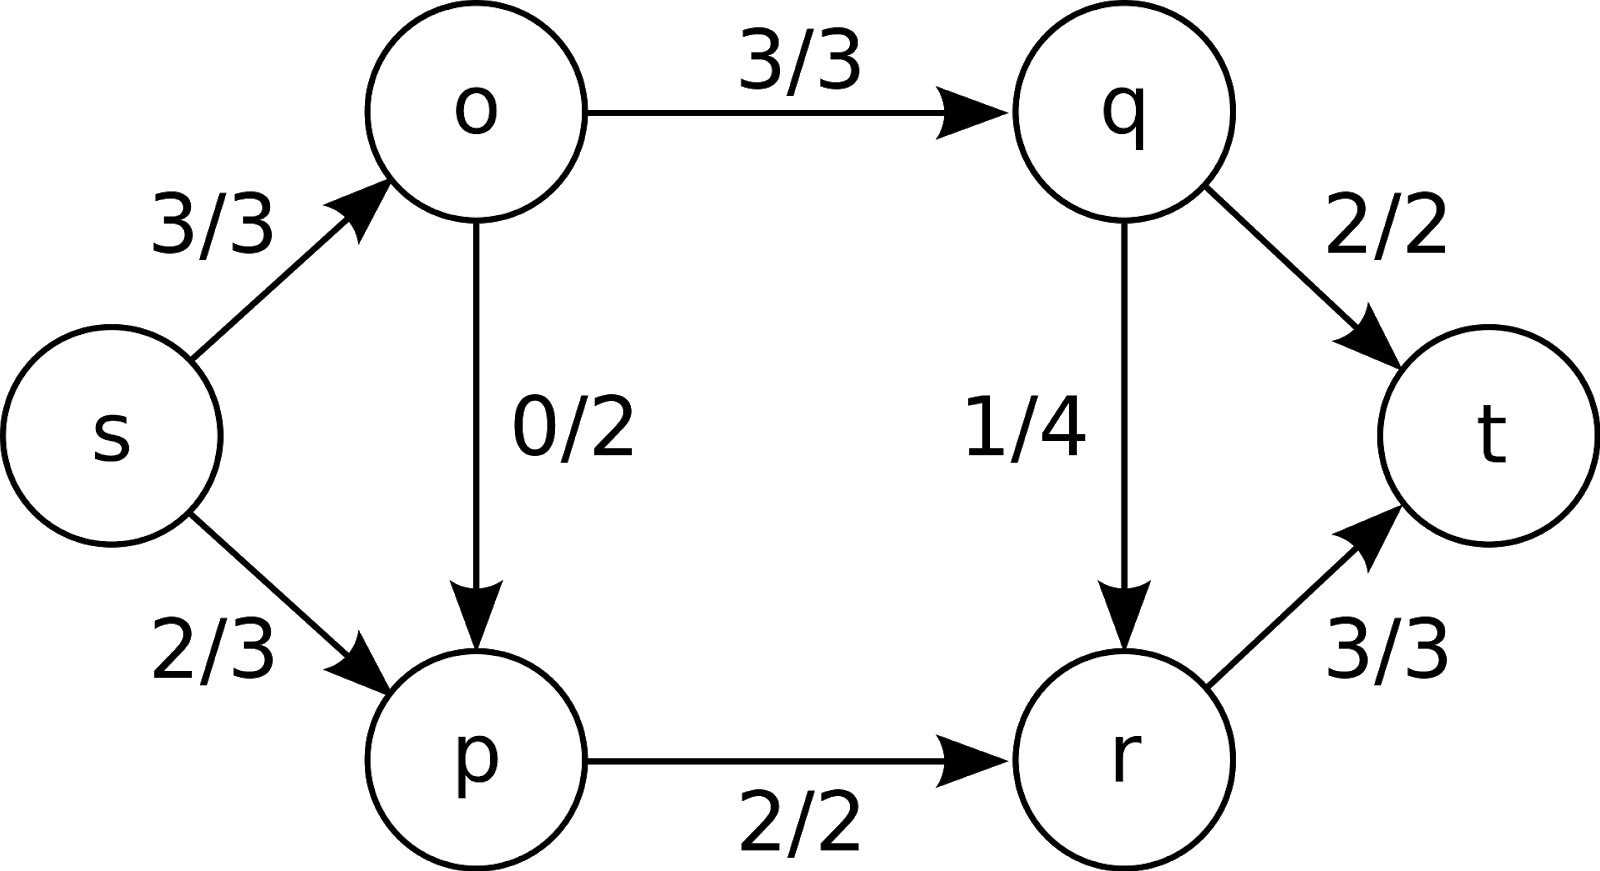
\includegraphics[width=7cm]{asset/example.png}
\end{center}
\end{frame}

\begin{frame}
\frametitle{Residual capacity}
\begin{itemize}
  \item \newTerm{Residual capacity} (kapasitas tersisa) dari setiap \fedge adalah sisa kapasitas \fedge tersebut, yaitu kapasitas awal dikurangi banyaknya aliran.
  \item Selain \fedge yang terdapat pada \fgraph awal, kita juga menambahkan \fbackEdge dengan arah kebalikan, dengan kapasitas sama dengan banyaknya aliran \fedge tersebut.
  \item \fBackEdge untuk mengembalikan aliran yang sudah dikirim sebelumnya (mengurangi banyaknya aliran pada \fedge). Bagian ini akan lebih jelas pada contoh metode Ford Fulkerson di bawah.
\end{itemize}
\end{frame}

\begin{frame}
\frametitle{Contoh residual capacity}
Sebagai contoh, \fgraph di gambar kiri merupakan banyaknya aliran dan kapasitas setiap \fedge, sedangkan graph di gambar kanan merupakan \fresidualCapacity setiap \fedge.
\newline
\begin{center}
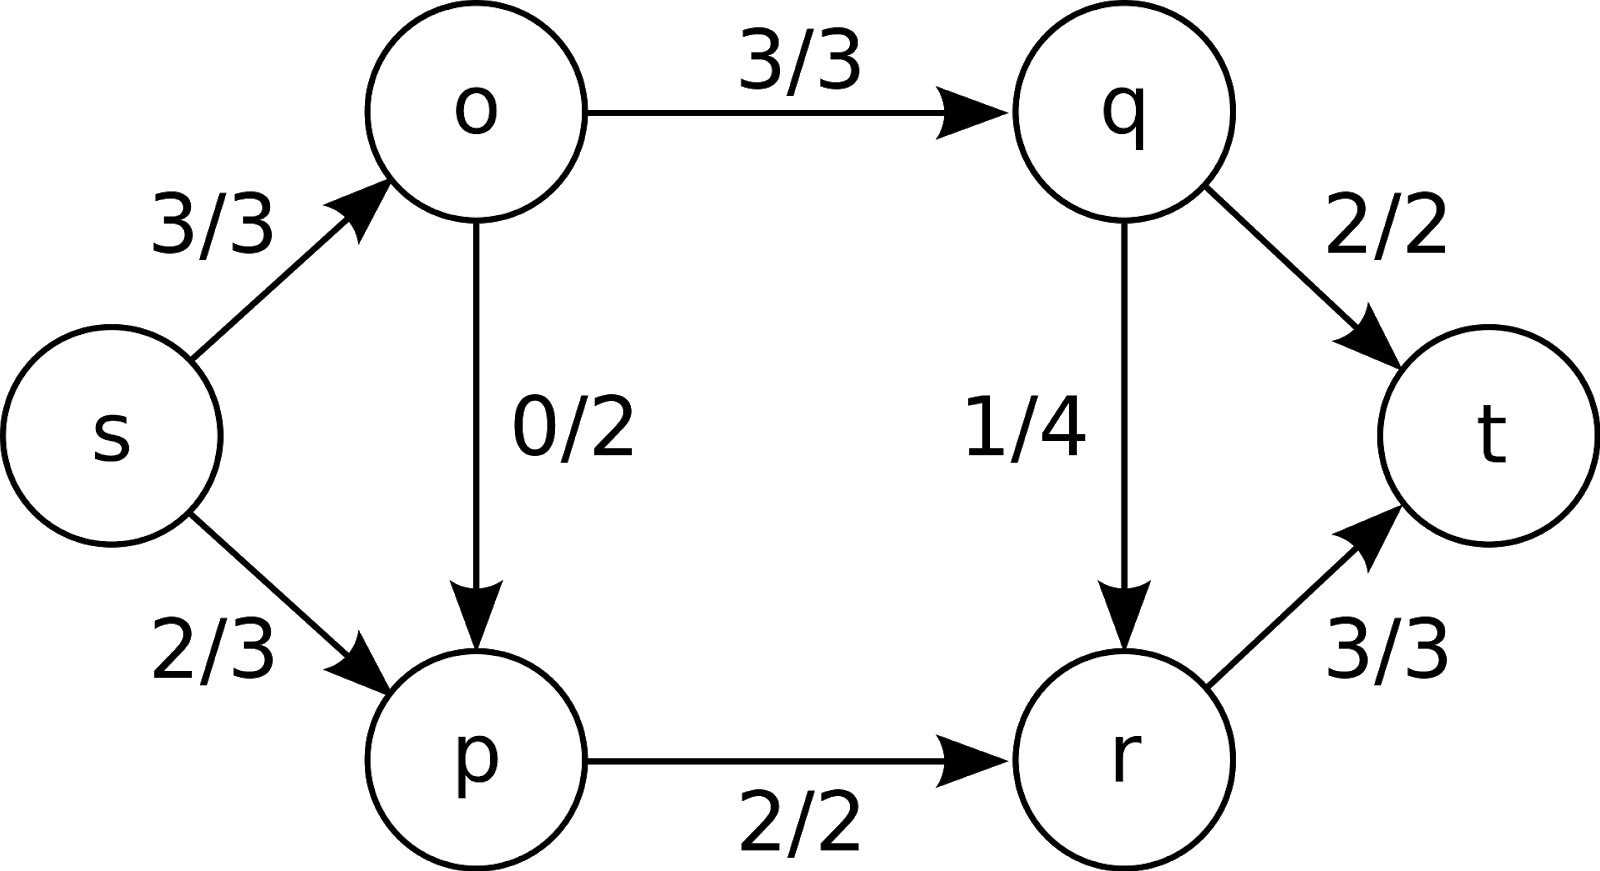
\includegraphics[width=5cm]{asset/example.png}
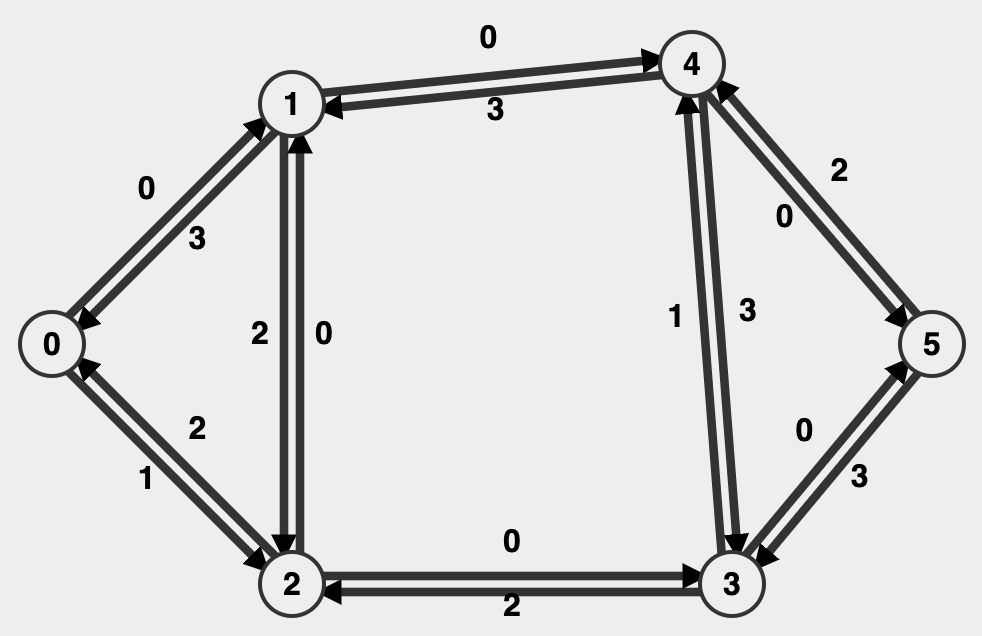
\includegraphics[width=5cm]{asset/residual-capacity.png}
\end{center}
\end{frame}

\begin{frame}
\frametitle{Metode Ford Fulkerson}
\begin{itemize}
  \item Metode \newTerm{Ford Fulkerson} mencari \newTerm{augmenting path} (sebuah \fpath yang melewati \fedge dengan \fresidualCapacity positif) secara terus menerus, dan menambahkan aliran melalui \fpath tersebut.
  \item Kita dapat menambahkan aliran sebanyak \newTerm{bottleneck} (\fresidualCapacity terkecil dari seluruh \fedge yang dikunjungi) dari \fpath tersebut, sehingga nilai \fmaxflow dapat ditambahkan dengan banyaknya aliran.
  \item Untuk seluruh \fedge $(u, v)$ yang dikunjungi oleh \fpath, kita harus mengurangi \fresidualCapacity \fedge $(u, v)$ dengan banyaknya aliran dan menambahkan \fresidualCapacity \fedge $(v, u)$ (\fbackEdge) dengan banyaknya aliran.
\end{itemize}
\end{frame}

\begin{frame}
\frametitle{Contoh Ford Fulkerson}
Sebagai contoh, diberikan \fgraph berikut, dengan \fnode $A$ sebagai \fsource dan \fnode $G$ sebagai \fsink.
\newline
\begin{center}
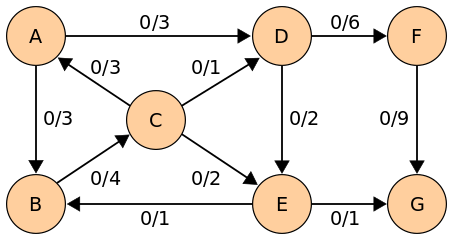
\includegraphics[width=7cm]{asset/ford-example-0.png}
\end{center}
\end{frame}

\begin{frame}
\frametitle{Contoh Ford Fulkerson (lanj.)}
Berikut adalah salah satu \faugmentingPath, melewati \fnode $A$, $D$, $E$, dan $G$. \fBottleneck dari \fpath ini adalah $1$ (\fedge $(E, G)$), sehingga nilai \fmaxflow kita tambahkan dengan $1$ dan memperbaharui \fresidualCapacity setiap \fedge yang dilewati.
\newline
\begin{center}
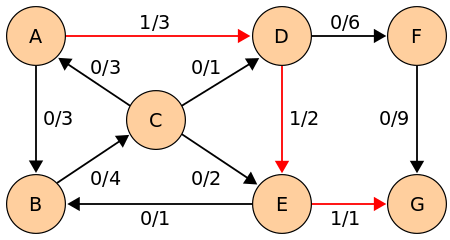
\includegraphics[width=7cm]{asset/ford-example-1.png}
\end{center}
\end{frame}

\begin{frame}
\frametitle{Contoh Ford Fulkerson (lanj.)}
Masih terdapat \faugmentingPath, salah satunya yang melewati \fnode $A$, $D$, $F$, dan $G$. \fBottleneck dari \fpath ini adalah $2$ (edge $(A, D)$), sehingga kita menambahkan nilai \fmaxflow dengan $2$. \fMaxflow sekarang adalah $3$.
\newline
\begin{center}
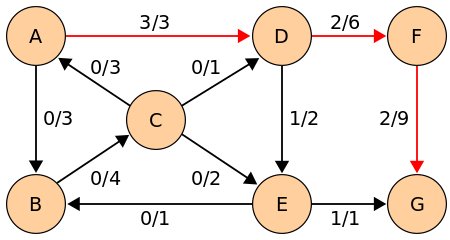
\includegraphics[width=7cm]{asset/ford-example-2.png}
\end{center}
\end{frame}

\begin{frame}
\frametitle{Contoh Ford Fulkerson (lanj.)}
Masih terdapat \faugmentingPath lagi, salah satunya yang melewati \fnode $A$, $B$, $C$, $D$, $F$, dan $G$. \fBottleneck dari \fpath ini adalah $1$ (\fedge $(C, D)$), sehingga kita menambahkan nilai \fmaxflow dengan $1$. \fMaxflow sekarang adalah $4$.
\newline
\begin{center}
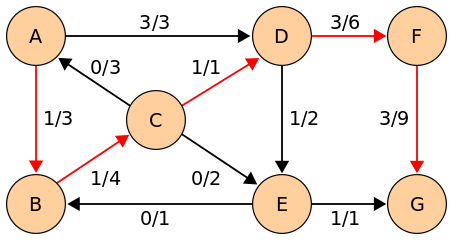
\includegraphics[width=7cm]{asset/ford-example-3.png}
\end{center}
\end{frame}

\begin{frame}
\frametitle{Contoh Ford Fulkerson (lanj.)}
Masih terdapat \faugmentingPath lagi. \fAugmentingPath ini memanfaatkan \fbackEdge $(D, E)$ dengan \fresidualCapacity $1$. \fAugmentingPath ini mengembalikan aliran yang melewati \fedge $(D, E)$ (aliran pertama) dan menggantinya untuk melewati \fedge $(D, F)$.
\newline
\begin{center}
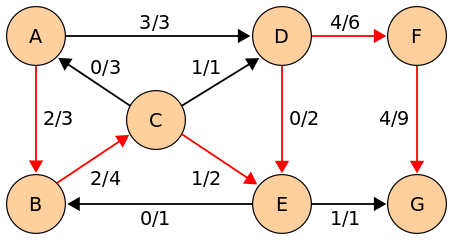
\includegraphics[width=7cm]{asset/ford-example-4.png}
\end{center}
\end{frame}

\begin{frame}
\frametitle{Contoh Ford Fulkerson (lanj.)}
\fBottleneck dari \faugmentingPath terakhir adalah $1$ (\fbackEdge $(D, E)$), sehingga kita menambahkan nilai \fmaxflow dengan $1$. \fMaxflow sekarang adalah $5$.
\newline
Tidak terdapat lagi \faugmentingPath, sehingga nilai \fmaxflow adalah $5$.
\newline
\begin{center}
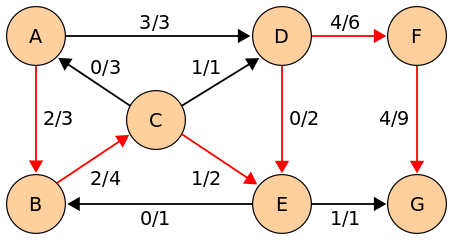
\includegraphics[width=7cm]{asset/ford-example-4.png}
\end{center}
\end{frame}

\begin{frame}
\frametitle{Mencari Augmenting Path}
\begin{itemize}
  \item Jika pencarian \faugmentingPath dilakukan dengan DFS, maka kompleksitas solusinya adalah $O(E * |f|)$, dengan $|f|$ adalah nilai \fmaxflow.
  \item Ini disebabkan karena sekali pencarian \faugmentingPath membutuhkan waktu $O(E)$ dan dapat menambahkkan $1$ pada nilai \fmaxflow.
  \item Berikut contoh \fgraph yang memerlukan $|f|$ pencarian \faugmentingPath.
\end{itemize}
\begin{center}
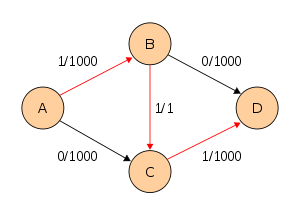
\includegraphics[width=5cm]{asset/ford-blowup-1.png}
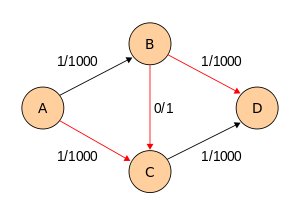
\includegraphics[width=5cm]{asset/ford-blowup-2.png}
\end{center}
\end{frame}

\begin{frame}
\frametitle{Algoritme Edmonds-Karp}
\begin{itemize}
  \item Algoritme \newTerm{Edmonds-Karp} adalah implementasi metode Ford Fulkerson dengan menggunakan BFS untuk mencari \faugmentingPath.
  \item Jika kita menggunakan BFS untuk mencari \faugmentingPath (yang akan mengembalikan \faugmentingPath dengan menggunakan paling sedikit \fedge), maka kita hanya akan mencari paling banyak $min(O(VE), |f|)$ \faugmentingPath.
  \item Sehingga kompleksitas waktu dari algoritme ini adalah $O(min(|V||E|^2, |E| \times |f|))$.
\end{itemize}
\end{frame}

\begin{frame}
\frametitle{Variasi Maximum Flow: Minimum Cut}
\begin{itemize}
  \item Diberikan sebuah \foreignTerm{weighted directed graph}\xspace dengan salah satu \fnode diberi label $s$ dan salah satu \fnode lainnya diberi label $t$.
  \item Persoalan \newTerm{minimum cut} adalah persoalan membagi himpunan \fnode menjadi dua buah subhimpunan \fnode $S$ dan $T$ (dengan $s \in S$ dan $t \in T$) yang meminimumkan total bobot perpotongan, yaitu $\sum_{u \in S} \sum_{v \in T} w(u, v)$.
  \item Teorema \newTerm{max-flow min-cut} menyatakan bahwa nilai \fmincut ini sama dengan nilai \fmaxflow dengan \fsource $s$ dan \fsink $t$.
\end{itemize}
\end{frame}

\begin{frame}
\frametitle{Variasi Maximum Flow: Lebih dari satu source/sink}
\begin{minipage}[\textheight]{\textwidth}
\begin{columns}[T]
\begin{column}{0.55\textwidth}
\begin{itemize}[]
  \item Jika terdapat lebih dari satu \fsource/\fsink, maka kita dapat menambahkan dua \fnode baru, super \fsource dan super \fsink, lalu menghubungkan super \fsource ke seluruh \fsource dan seluruh \fsink ke super \fsink (dengan kapasitas tak terhingga).
  \item Jalankan algoritme \fmaxflow dengan memilih super \fsource sebagai \fsource dan super \fsink sebagai \fsink.
\end{itemize}
\end{column}
\begin{column}{0.45\textwidth}
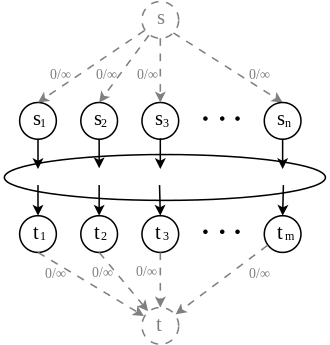
\includegraphics[width=5cm]{asset/multiple-source-sink.png}
\end{column}
\end{columns}
\end{minipage}
\end{frame}

\begin{frame}
\frametitle{Variasi Maximum Flow: Kapasitas Node}
\begin{minipage}[\textheight]{\textwidth}
\begin{columns}[T]
\begin{column}{0.6\textwidth}
\begin{itemize}[]
  \item Jika setiap \fnode juga memiliki kapasitas banyaknya aliran yang dapat melewati \fnode tersebut, maka kita dapat memisahkan \fnode tersebut menjadi dua \fnode dan menambahkan \fedge yang menghubungkan keduanya dengan kapasitas \fnode tersebut.
  \item Sebagai contoh, jika \fnode $v$ pada gambar di samping (atas) memiliki kapasitas $2$, maka kita dapat memisahnya seperti gambar di samping (bawah)
\end{itemize}
\end{column}
\begin{column}{0.4\textwidth}
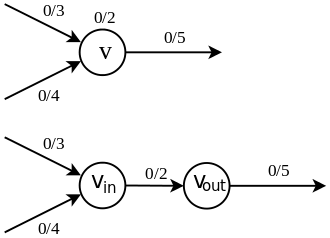
\includegraphics[width=4.5cm]{asset/node-capacity.png}
\end{column}
\end{columns}
\end{minipage}
\end{frame}

\begin{frame}
\frametitle{Contoh Aplikasi: COCI 2017/2018 Round \#7 (PRIGLAVCI)}
\begin{itemize}
  \item Terdapat $N$ murid dan $M$ halte pada koordinat 2 dimensi.
  \item Terdapat $K$ rute bus yang melewati beberapa halte. Hanya terdapat 1 bus pada setiap rute.
  \item Setiap bus dapat berisi maksimal $C$ murid.
  \item Setiap murid dapat naik bus dari halte manapun di suatu rute, namun hanya dapat turun dari bus di halte terakhir rute tersebut.
  \item Kita ingin mengatur setiap murid harus naik bus dari halte mana, sehingga kapasitas bus mencukupi untuk semua murid dan ``kelemahan''-nya minimum.
  \item ``Kelemahan'' suatu pengaturan didefinisikan sebagai jarak Euclidean yang paling maksimum antara seorang murid ke halte yang harus dikunjunginya.
\end{itemize}
\end{frame}

\begin{frame}
\frametitle{Solusi: COCI 2017/2018 Round \#7 (PRIGLAVCI)}
\begin{itemize}
  \item Kita dapat menyelesaikan soal ini menggunakan Binary Search the Answer
  \item Untuk setiap $x$, kita dapat memeriksa apakah terdapat solusi dengan “kelemahan” tidak lebih dari $x$ dengan cara mengkonstruksi \fgraph berikut:
  \begin{itemize}
    \item Tambahkan satu node untuk setiap murid, rute, dan halte.
    \item Tambahkan \fnode \fsource dan \fsink.
    \item Tambahkan \fedge dari \fsource ke setiap murid dengan kapasitas $1$.
    \item Tambahkan \fedge dari setiap rute ke \fsink dengan kapasitas $C$.
    \item Untuk setiap murid $m$ dan rute $r$, jika terdapat halte $h$ pada rute $r$ dengan jarak Euclidean dari murid $m$ ke halte $h$ tidak lebih dari $x$, maka tambahkan \fedge dari murid $m$ ke rute $r$ dengan kapasitas $1$.
  \end{itemize}
\end{itemize}
\end{frame}

\begin{frame}
\frametitle{Solusi: COCI 2017/2018 Round \#7 (PRIGLAVCI) (lanj.)}
\begin{itemize}
  \item Jika nilai \fmaxflow dari \fgraph yang dikonstruksi adalah $N$, maka terdapat pemetaan untuk setiap siswa ke rute bis, dengan jarak Euclidean murid dan halte tempat murid tersebut naik bis tidak lebih dari $x$, dan seluruh bis tidak melebihi kapasitasnya.
  \begin{itemize}
    \item Dalam kasus ini, kita dapat mencoba untuk menurunkan nilai $x$ pada binary search.
  \end{itemize}
  \item Kita dapat menginterpretasikan sebuah aliran dari \fsource $\rightarrow$ murid $m$ $\rightarrow$ rute $r$ $\rightarrow$ \fsink sebagai murid $m$ mengambil rute $r$.
\end{itemize}
\end{frame}



\end{document}
